\subsubsection{Limitation}

Prediction cost in baseline method consists of following two parts.

\begin{enumerate}
	\item Search cost for the cell which contains the key. This cost will be equal to $log_{2}N_{1}$, where $N_{1}$ is the number of cells into which mapped values are divided.
	
	\item Cost associated with sequentially comparing the query point key value against keys inside the cell found in previous search. On average this cost will be equal to $N_{2}\div2$, where $N_{2}$ is the number of keys in a cell.   
	
If cell size is large, number of cells will be smaller, number of keys per cell will be higher, resulting in higher cost of sequential scan with in the cell. 
\end{enumerate}
Consider the example in figure \ref{fig:BaseLine_Method_Limitation}. Dataset is divided into 3 sections based on the mapped values. Any point or range query in the second triangle(page) will result into a sequential scan through all 9 keys in the cells.

\begin{figure*}[t]
    \centering
    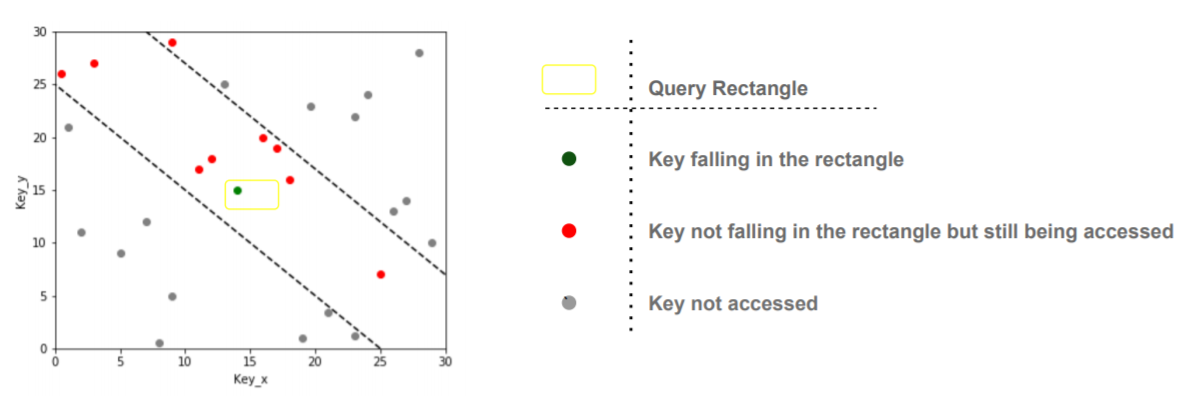
\includegraphics[width=1\textwidth]{graphs/Lisa_Baseline_Model_Limitation.png}
    \caption{Baseline Method Limitation }
    \label{fig:BaseLine_Method_Limitation}
\end{figure*}
